\section{Co-rotinas} 
\label{sec:co_rotinas}
Co-rotinas são um tipo especial de subprogramas. A linguagem Lua é uma das linguagens que possui co-rotinas. Co-rotinas possuem múltiplos pontos de entrada controlados elas mesmas. A cada execução (chamado de resumo), a co-rotina volta a sua execução não do início, mas sim de algum outro ponto (por isso resumo). Co-rotinas mantém seu estado entre as ativações e portanto são sensíveis ao histórico, ou seja, possuem variáveis estáticas.

Geralmente, corrotinas são criadas pela aplicação por uma unidade chamada de unidade mestre. A unidade mestre não é uma co-rotina, é tem a função de ativar uma das co-rotinas, que após suas inicializações, resumem uma as outras até que a execução de todas termine e o controle volte para a unidade mestre. As figuras \ref{co-rotinas} e \ref{co-rotinas_b} ilustram o possível funcionamento de duas co-rotinas A e B.

\begin{figure}[ht!]
 \centering
 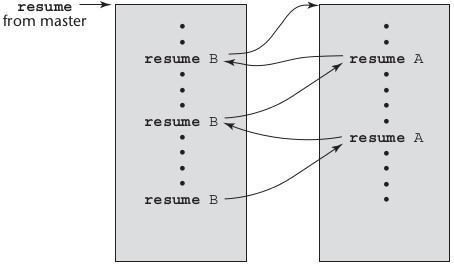
\includegraphics[scale=0.65]{./imagens/coroutines.png}
 \caption{Execução de co-rotinas 1 \cite{sebesta}}
\label{co-rotinas}
\end{figure}

\begin{figure}[ht!]
 \centering
 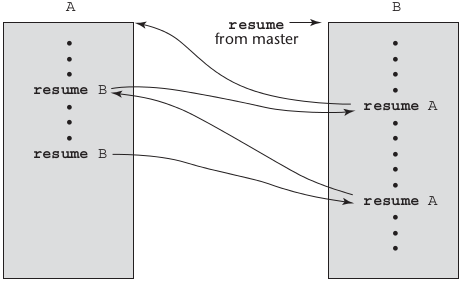
\includegraphics[scale=0.65]{./imagens/coroutines_b.png}
 \caption{Execução de co-rotinas 2 \cite{sebesta}}
\label{co-rotinas_b}
\end{figure}
